\section{Methodology}

\textsc{Date} describes the density-based clustering analysis which is a novel contribution of this work. This process attempts to map data to a three-dimensional space, then use spatial features to generate hidden features.

\subsection{Point Cloud Creation}
Point clouds are a set of Cartesian coordinates $(x, y, z)$ which represent some points in a three-dimensional space. Point clouds may be used in computer vision software as a method for mapping high-dimensional shapes into lower-dimensional space~\cite{Wang_2019_ICCV}. As a latent representation, this method can be used temporally to express the movement of objects in three-dimensional space. An airplane can be modeled as a three-dimensional point cloud, and its movement described as a series of clouds ${c_0, c_1,...,c_t}$ where $t$ represents a number of time intervals and $c_n$ the point cloud generated at a given time slice. Like the work of Quach et al~\cite{Quach2020compression}, we do not combine multiple representations in a time series but instead analyze the static representations much analagous to manifolds in three-dimensional space. We use the geometrical representation captured here for cluster analysis.

\begin{figure} [ht!]
\centering
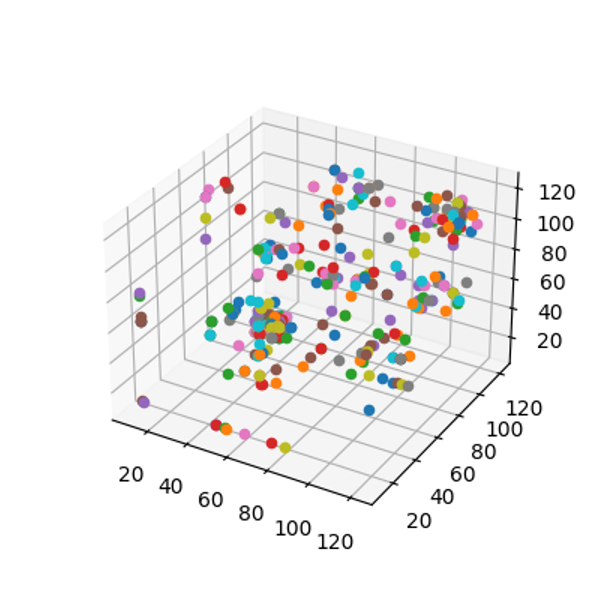
\includegraphics[width=0.6\textwidth]{chapters/6/img/sipcloud.png}
\caption{3D point cloud made out of a Session Initiation Protocol (SIP) packet.}
\label{fig:cloud}
\end{figure}

In the \textsc{Date} model, payload data is extracted from the packets and truncated to 1024 bytes. If the payload is shorter than this, we add padding for normalization. Byte values $v$ are converted to decimal values $v' \in [0,255]$. For example, the byte string, `0x68', `0x65', `0x6c', `0x6c', `0x6f', would first be transformed to decimal values (104, 101, 108, 108, 111). Then, the sliding window would produce the points corresponding to coordinates:
\begin{equation}
\begin{split}
     C =
\{(104, 101, 108), \\ (101, 108, 108), \\ (108, 108, 111)\}.
\end{split}
\end{equation}

The coordinates are mapped to a three-dimensional space to form point clouds like Figure~\ref{fig:cloud}. We expect that similar point clouds will be generated from packets with similar data.


\subsection{Density-Based Spatial Clustering of Applications With Noise (DBSCAN)}

Density-Based Spatial Clustering of Applications with Noise (DBSCAN) uses three different point classifications. \textit{Core points} make up the centers of clusters. Individual core points are labeled based on the number of neighbors they have compared to their neighbors, or their degree of importance. \textit{Border points} are those which have the least number of neighbors but are still comparatively relevant due to being within the range of a core point. These comprise the edges of the point cloud. \textit{Outlier points} are neither borders nor cores, do not belong to a cluster, and are considered noise~\cite{schubert2017dbscan}. The DBSCAN algorithm visits each point and classifies them as such in order to paint a picture of where clusters of data are as in Figure~\ref{fig:dbscan}.

\begin{figure} [ht!]
\centering
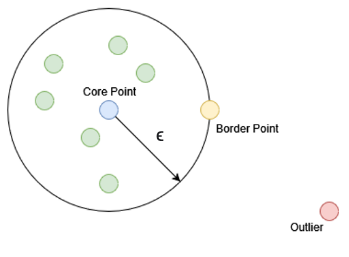
\includegraphics[scale=0.4]{chapters/6/img/dbscan.drawio.png}
\caption{Illustration of types of points in DBSCAN.}
\label{fig:dbscan}
\end{figure}

We first create the point clouds and then process them using DBSCAN in order to derive the natural clusters that exist in the data. DBSCAN groups points that are close together utilizing a Euclidean distance for measurements. The value of the Euclidean distance that determines proximity and the minimum number of points needed to form a cluster are configurable parameters: $\epsilon$ and a minimum number of samples. The $\epsilon$ value is the radius for each circle drawn around each point to query density, and the minimum number of samples is the minimum number of points required to be inside the drawn circle for it to be considered a Core point.

Generally, the number of samples is twice the dimensions, but it must be at least the number of dimensions. If it is set below this threshold, then singular points or two points that are close together would constitute a cluster, which would not be an accurate way of determining where data is clumped~\cite{mullin2020tuning}. In our experiments, we configured DBSCAN to perform with $\epsilon$ = 7 and \texttt{min\_samples} = 7. This would be enough to create more clusters in a less populated point cloud. An $\epsilon$ value of 7 also allowed for a greater number of recognizable clusters~\cite{rahmah2016determination}.

Like many machine learning models, the parameters used to tune DBSCAN greatly affect performance rates. It is possible to create more clearly defined point clouds within the three-dimensional space through this parameter adjustments. The $\epsilon$ value needs to be set based on general rules. If the value of $\epsilon$ chosen is too small then too many clusters will be created which over-emphasize the importance of noisy points. However, if set too large, then clusters will merge together and shapes become less distinct. One way that a value of $\epsilon$ can be estimated is by examining the input data and finding the average distance between each point and its $K$-nearest neighbors. Choosing an exact value for $\epsilon$ is a difficult problem for packet data which is highly variable. The $\epsilon$ value must be estimated from a conglomeration of the packet's $K$-nearest neighbors where $K$ is equal to \texttt{min\_samples}.

Because each packet is highly variable, choosing an exact value for $\epsilon$ is a difficult problem. An estimation of $\epsilon$ must be taken from a conglomeration of the packet's $k$-nearest neighbors data where $k$ is the value of \texttt{min\_samples} chosen. As shown in the figure above, the point of each line with the greatest curvature is considered the ideal value for $\epsilon$. A line has been illustrated in Figure~\ref{fig:kneighborsgraph} where an estimated average is made for every sample. The variation in an ideal $\epsilon$ value could be a major factor in why some packets are recognizable in their cloud state and others are not~\cite{rahmah2016determination}.

We extract the following features as the feature vector for classification from the DBSCAN results:
\begin{itemize}
    \item clusterCount = number of clusters
    \item averageClusterSize = average cluster size
    \item standardDeviation = standard deviation
    \item noisePercent = percent of cloud containing noise
\end{itemize}

\begin{figure} [ht!]
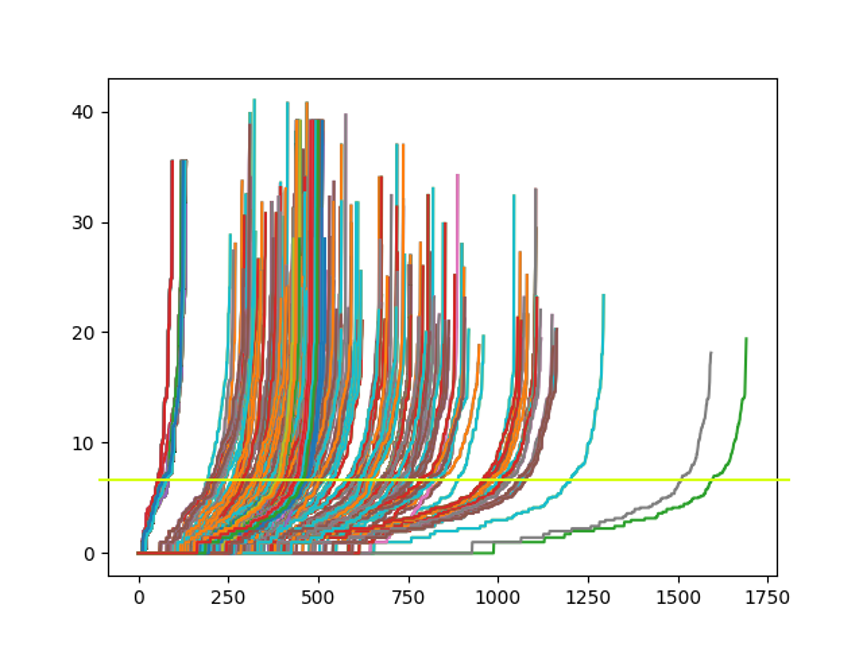
\includegraphics[width=\linewidth]{chapters/6/img/kmembersgraph.png}
\caption{K-nearest neighbors graph generated for packets in the dataset using a \texttt{min\_samples} = 6.}
\label{fig:kneighborsgraph}
\end{figure}

\subsection{Packet Classification}
For deep learning, we feed the extracted cluster features forward into a two-layer multilayer perceptron unit (MLP) with a final softmax layer for classification. We use binary cross entropy as the loss function.
